\chapter{Lampiran A. Tangkapan Layar Hasil Pengujian}

\begin{figure}[!htb]
	\centering
	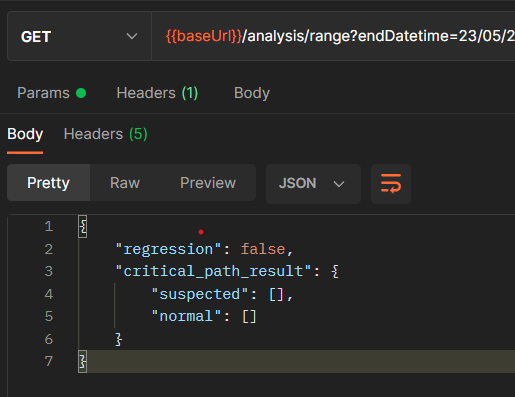
\includegraphics[width=0.75\textwidth]{resources/ch4/json/1.png}
	\caption{\textit{Response} JSON hasil pengujian kasus \textbf{SI1}}
	\label{result_json_1}
\end{figure}

\begin{figure}[!htb]
	\centering
	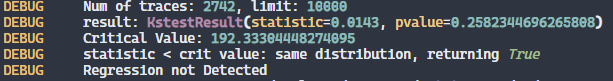
\includegraphics[width=1\textwidth]{resources/ch4/log/1-log.png}
	\caption{\textit{Log} hasil pengujian kasus SI1}
	\label{result_log_1}
\end{figure}

\begin{figure}[!htb]
	\centering
	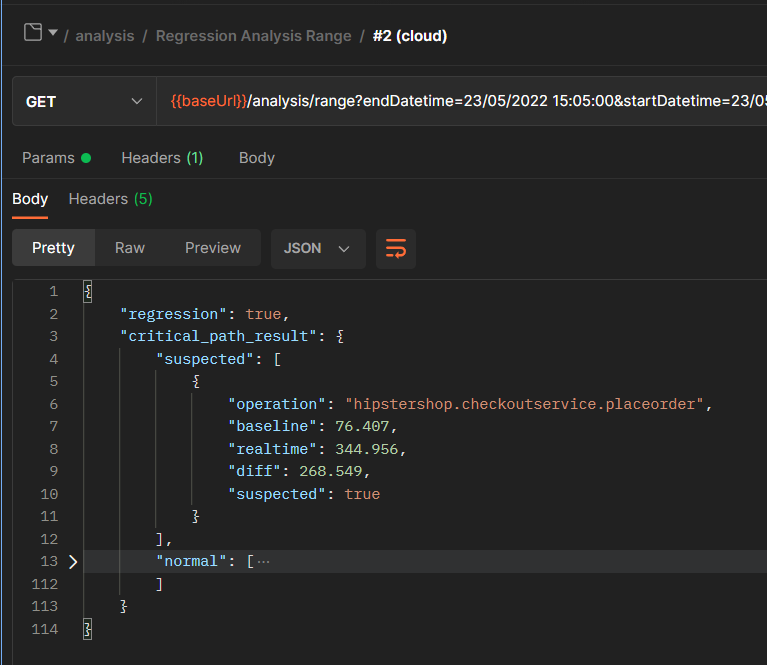
\includegraphics[width=0.75\textwidth]{resources/ch4/json/2.png}
	\caption{\textit{Response} JSON hasil pengujian kasus \textbf{SI2}}
	\label{result_json_2}
\end{figure}

\begin{figure}[!htb]
	\centering
	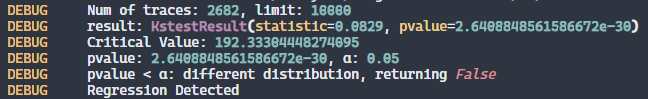
\includegraphics[width=1\textwidth]{resources/ch4/log/2-log.png}
	\caption{\textit{Log} hasil pengujian kasus SI2}
	\label{result_log_2}
\end{figure}